\begin{figure}[ht]
\centering
% Thesis-wide categorical color palette
% Usage: % Thesis-wide categorical color palette
% Usage: % Thesis-wide categorical color palette
% Usage: \input{figures/palette} in any figure file
%
% Muted primary colors -- print-friendly, visually distinct.
% Inspired by Cooper Union's red/blue primaries, softened for
% academic figures. Use palA-palC for data series in scatter
% plots, line charts, bar charts, etc.

\definecolor{palA}{HTML}{1F77B4}   % Tableau blue
\definecolor{palB}{HTML}{D62728}   % Tableau red
\definecolor{palC}{HTML}{2CA02C}   % Tableau green
 in any figure file
%
% Muted primary colors -- print-friendly, visually distinct.
% Inspired by Cooper Union's red/blue primaries, softened for
% academic figures. Use palA-palC for data series in scatter
% plots, line charts, bar charts, etc.

\definecolor{palA}{HTML}{1F77B4}   % Tableau blue
\definecolor{palB}{HTML}{D62728}   % Tableau red
\definecolor{palC}{HTML}{2CA02C}   % Tableau green
 in any figure file
%
% Muted primary colors -- print-friendly, visually distinct.
% Inspired by Cooper Union's red/blue primaries, softened for
% academic figures. Use palA-palC for data series in scatter
% plots, line charts, bar charts, etc.

\definecolor{palA}{HTML}{1F77B4}   % Tableau blue
\definecolor{palB}{HTML}{D62728}   % Tableau red
\definecolor{palC}{HTML}{2CA02C}   % Tableau green

\definecolor{nodeblue}{HTML}{B8D2E6}
\definecolor{nodeborder}{HTML}{5A87B5}
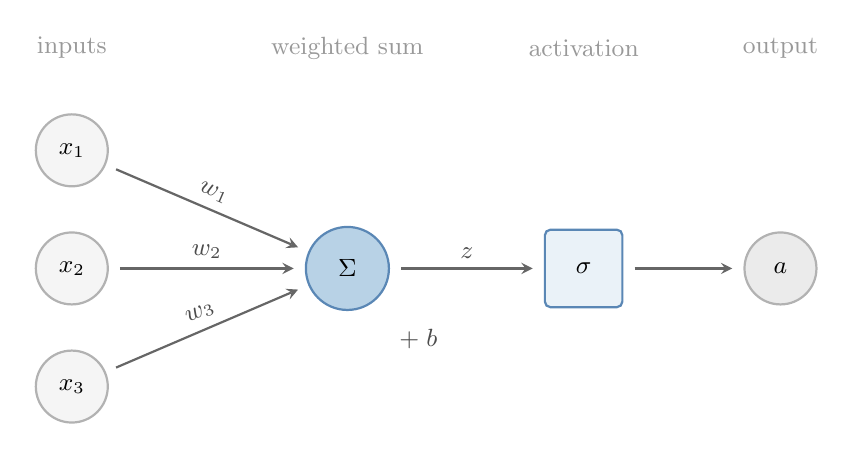
\begin{tikzpicture}[
    inputnode/.style={circle, draw=black!30, thick, fill=black!4,
                      minimum size=26pt, inner sep=0pt},
    sumnode/.style={circle, draw=nodeborder, thick, fill=nodeblue,
                    minimum size=30pt, inner sep=0pt},
    actnode/.style={rectangle, draw=nodeborder, thick, fill=nodeblue!30,
                    minimum width=28pt, minimum height=28pt,
                    inner sep=2pt, rounded corners=2pt},
    outputnode/.style={circle, draw=black!30, thick, fill=black!8,
                       minimum size=26pt, inner sep=0pt},
    conn/.style={->, thick, >=stealth, black!60},
    mathlbl/.style={font=\small, text=black!70},
    seclbl/.style={font=\small, text=black!40},
]

% --- Input nodes (math variable inside) ---
\node[inputnode] (x1) at (0, 1.5)  {\small $x_1$};
\node[inputnode] (x2) at (0, 0)    {\small $x_2$};
\node[inputnode] (x3) at (0, -1.5) {\small $x_3$};

% --- Summation node ---
\node[sumnode] (sum) at (3.5, 0) {\small $\Sigma$};

% --- Bias label (below-right of sum node) ---
\node[mathlbl] at (4.4, -0.9) {$+\; b$};

% --- Connections with weight labels ---
\draw[conn, shorten >=4pt, shorten <=4pt] (x1) -- (sum) node[mathlbl, midway, above, sloped] {$w_1$};
\draw[conn, shorten >=4pt, shorten <=4pt] (x2) -- (sum) node[mathlbl, midway, above, sloped] {$w_2$};
\draw[conn, shorten >=4pt, shorten <=4pt] (x3) -- (sum) node[mathlbl, midway, above, sloped] {$w_3$};

% --- Activation function ---
\node[actnode] (act) at (6.5, 0) {\small $\sigma$};
\draw[conn, shorten >=4pt, shorten <=4pt] (sum) -- (act) node[mathlbl, midway, above] {$z$};

% --- Output ---
\node[outputnode] (out) at (9.0, 0) {\small $a$};
\draw[conn, shorten >=4pt, shorten <=4pt] (act) -- (out);

% --- Section labels above ---
\node[seclbl] at (0, 2.8) {inputs};
\node[seclbl] at (3.5, 2.8) {weighted sum};
\node[seclbl] at (6.5, 2.8) {activation};
\node[seclbl] at (9.0, 2.8) {output};

\end{tikzpicture}
\caption{A single neuron. Each input is multiplied by a weight, the
  results are summed with a bias, and the total is passed through an
  activation function to produce the output.}
\label{fig:neuron}
\end{figure}
